\documentclass{article}%
\usepackage[T1]{fontenc}%
\usepackage[utf8]{inputenc}%
\usepackage{lmodern}%
\usepackage{textcomp}%
\usepackage{lastpage}%
\usepackage{geometry}%
\geometry{margin=0.7in}%
\usepackage{ragged2e}%
\usepackage{graphicx}%
\usepackage{fancyhdr}%
%
\fancypagestyle{header}{%
\renewcommand{\headrulewidth}{0pt}%
\renewcommand{\footrulewidth}{0pt}%
\fancyhead{%
}%
\fancyfoot{%
}%
\fancyhead[L]{%
Page date: %
\linebreak%
2023{-}02{-}04%
}%
\fancyhead[C]{%
Georgia Institute of Technology%
}%
\fancyhead[R]{%
Page \thepage\ of \pageref{LastPage}%
}%
}%
%
\begin{document}%
\normalsize%
\pagestyle{header}%
\begin{minipage}{\textwidth}%
\centering%
\begin{Large}%
\textbf{HW2: Problem 1}%
\end{Large}%
\linebreak%
\begin{large}%
\textbf{Ian Dover}%
\end{large}%
\end{minipage}%
\section{Part A}%
\label{sec:PartA}%
Image converted to greyscale:%


\begin{figure}[h!]%
\centering%
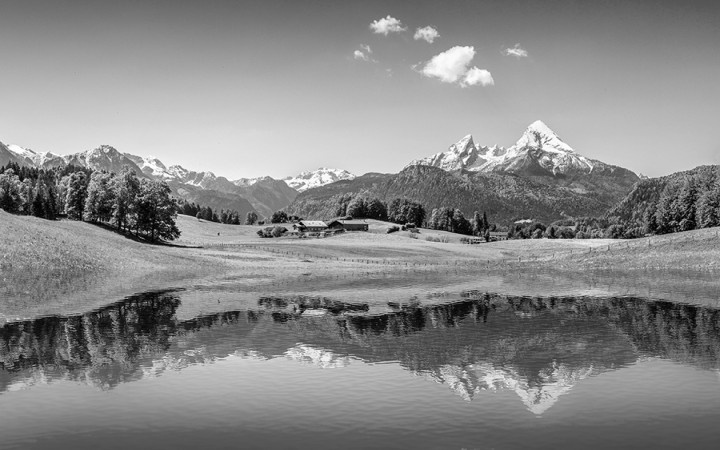
\includegraphics[width=120px]{/com.docker.devenvironments.code/reports/problem1/../../output/problem1/p1_a_grayscale.jpg}%
\caption{Greyscale image.}%
\end{figure}

%
\section{Part B}%
\label{sec:PartB}%
\subsection{Subsection 1}%
\label{subsec:Subsection1}%
Image with zero{-}mean Gaussian white noise with variance of 0.01:%


\begin{figure}[h!]%
\centering%
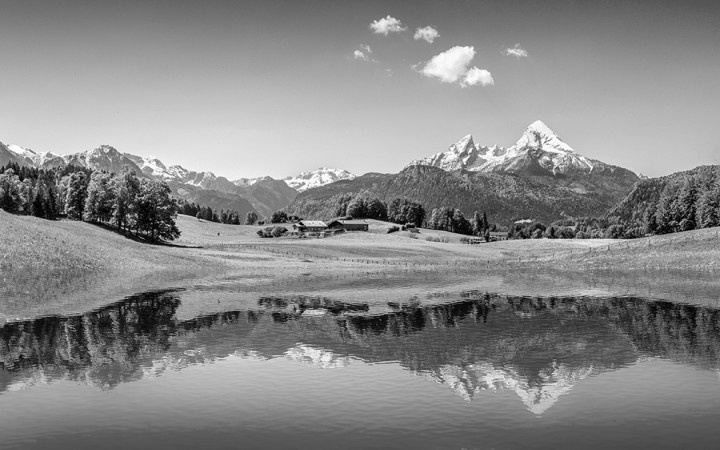
\includegraphics[width=120px]{/com.docker.devenvironments.code/reports/problem1/../../output/problem1/p1_b_1_gaussian.jpg}%
\caption{J1: Greyscale image with gaussian noise applied.}%
\end{figure}

%
\subsection{Subsection 2}%
\label{subsec:Subsection2}%
Image with salt{-}and{-}pepper noise, affecting approximately 5\% of pixels:%


\begin{figure}[h!]%
\centering%
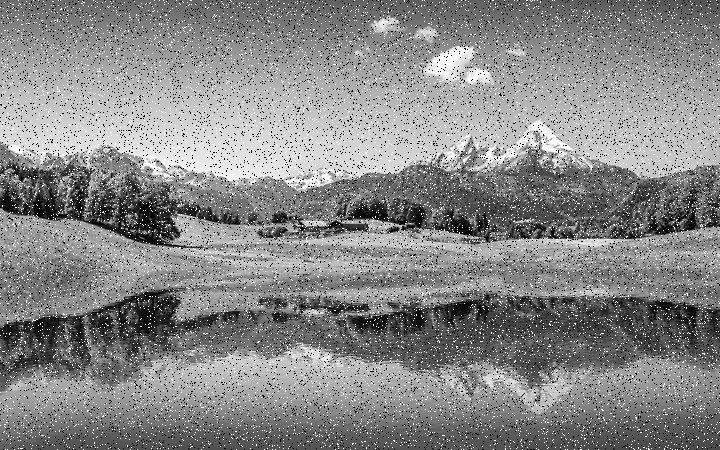
\includegraphics[width=120px]{/com.docker.devenvironments.code/reports/problem1/../../output/problem1/p1_b_2_salt_and_pepper.jpg}%
\caption{J2: Greyscale image with salt{-}and{-}pepper noise applied.}%
\end{figure}

%
\newpage%
\section{Part C}%
\label{sec:PartC}%
\subsection{Gaussian De{-}noise: J1}%
\label{subsec:GaussianDe{-}noiseJ1}%
Images with gaussian filter denoise on J1:%


\begin{figure}[h!]%
\centering%
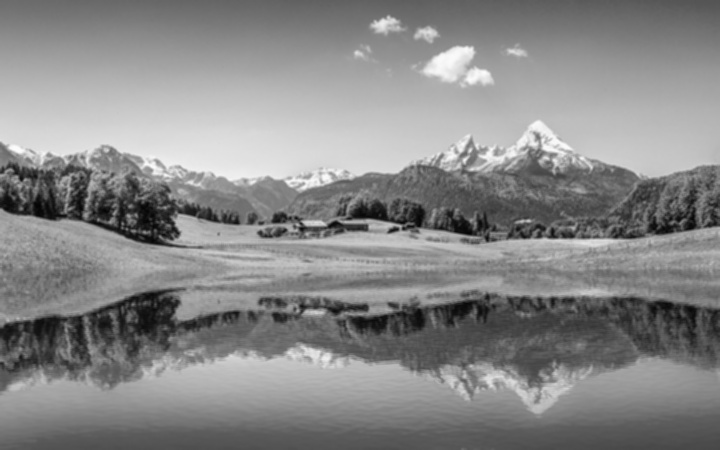
\includegraphics[width=120px]{/com.docker.devenvironments.code/reports/problem1/../../output/problem1/p1_c_1_j1.jpg}%
\caption{Gaussian filter denoised J1.}%
\end{figure}

%
\subsection{Gaussian De{-}noise: J2}%
\label{subsec:GaussianDe{-}noiseJ2}%
Images with gaussian filter denoise on J2:%


\begin{figure}[h!]%
\centering%
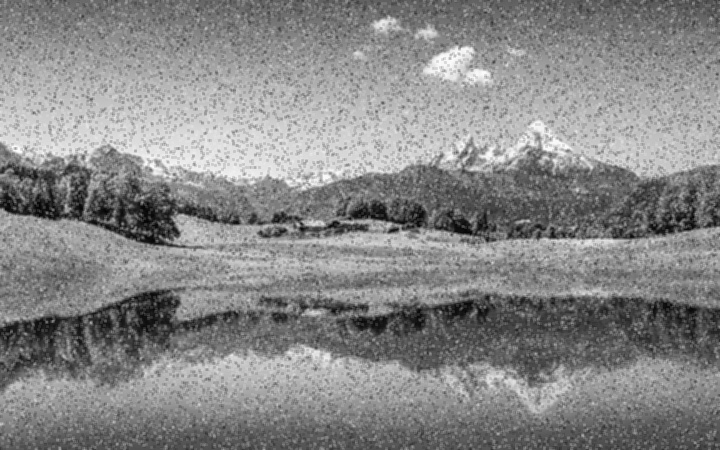
\includegraphics[width=120px]{/com.docker.devenvironments.code/reports/problem1/../../output/problem1/p1_c_1_j2.jpg}%
\caption{Gaussian filter denoised J2.}%
\end{figure}

%
\subsection{Median De{-}noise: J1}%
\label{subsec:MedianDe{-}noiseJ1}%
Images with median filter denoise on J1:%


\begin{figure}[h!]%
\centering%
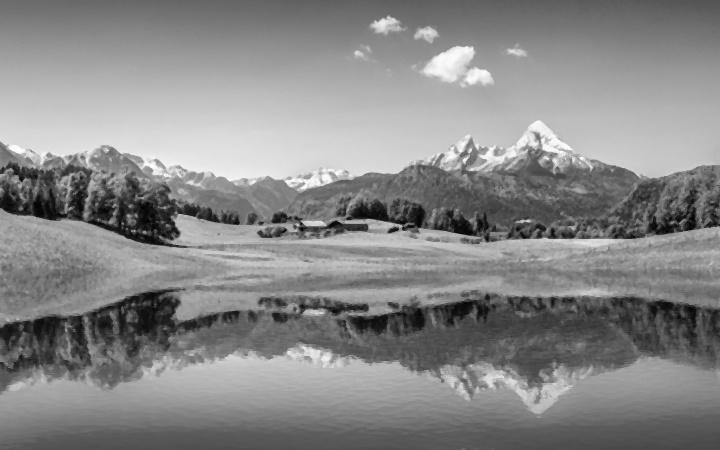
\includegraphics[width=120px]{/com.docker.devenvironments.code/reports/problem1/../../output/problem1/p1_c_2_j1.jpg}%
\caption{Median filter denoised J1.}%
\end{figure}

%
\subsection{Median De{-}noise: J2}%
\label{subsec:MedianDe{-}noiseJ2}%
Images with median filter denoise on J2:%


\begin{figure}[h!]%
\centering%
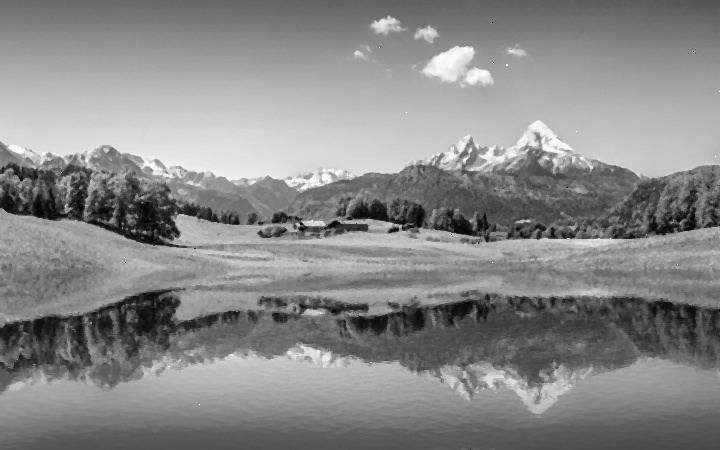
\includegraphics[width=120px]{/com.docker.devenvironments.code/reports/problem1/../../output/problem1/p1_c_2_j2.jpg}%
\caption{Median filter denoised J2.}%
\end{figure}

%
\end{document}